\section{Descrição geral dos algoritmos}

O GRASP segue um ciclo multi-start ilustrado pela Figura~\ref{fig:pseudogeral}. Em cada iteração, constrói-se uma solução viável, executa-se a busca local e atualiza-se a melhor solução global.

\begin{figure}[H]
\centering
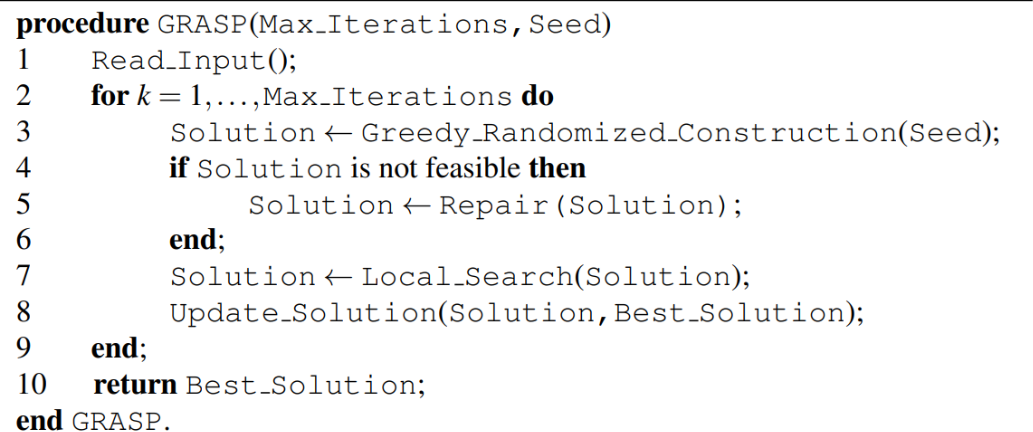
\includegraphics[width=0.72\textwidth]{imagens/pseudo-codigo-geral.png}
\caption{Pseudocódigo geral do GRASP adaptado à implementação.}
\label{fig:pseudogeral}
\end{figure}

A construção produz diversidade e a busca local intensifica a solução. No GRASP clássico, $\alpha$ permanece constante. No GRASP Reativo, as probabilidades de escolha dos valores de $\alpha$ são atualizadas ao fim de cada bloco, com base nos custos observados. A probabilidade de escolher um valor $\alpha$ é calculada por
\begin{equation}
p(\alpha)=
\frac{\left(F_{\mathrm{melhor}}/\bar F(\alpha)\right)^\delta}
{\displaystyle\sum_{\beta\in\mathcal{A}}
\left(F_{\mathrm{melhor}}/\bar F(\beta)\right)^\delta},
\end{equation}
em que $\bar F(\alpha)$ é o custo médio das soluções obtidas com $\alpha$, $F_{\mathrm{melhor}}$ é o menor custo encontrado até então e $\mathcal{A}$ é o conjunto de valores de $\alpha$. A normalização faz com que as probabilidades somem 1. O parâmetro $\delta=5$ controla a preferência por valores de $\alpha$ com melhor desempenho: quanto maior $\delta$, maior essa preferência. O ótimo conhecido da instância não é usado nesse cálculo.

A calibração seleciona um único $\alpha$ antes dos experimentos finais usando instâncias representativas. O GRASP Reativo, por sua vez, atualiza as probabilidades de uma grade de valores durante a execução.